
% \begin{textbox}{Key concepts I}
% \red{Bag-of-words (BOW)}

% \green{\emph{type} vs. \emph{token}}
% \emph{To be or not to be.} = 6 \emph{tokens}, 4 \emph{types}.

% \red{\emph{type}} descriptive criterion\footcite[cf.][12]{stroustrup}

% \red{\emph{token}} unit of analysis\footcites[cf.][12]{stroustrup,attentionMerchants}


% \bigskip

% \underline{Key topics}
% \begin{itemize}
%     \item One
%     \item Two
%     \item Three
% \end{itemize}

% \end{textbox}



\begin{textbox}{Check List}
\red{Have you checked}
\begin{enumerate}
    \item Connect all $V_{DD}$, $V_{SS}$, and $GND$?
    \item Pin 1 of a chip at the right location?
    \item Consume right amount of power (i.e., \emph{current})?
\end{enumerate}
    
\end{textbox}

\subsection{Connectivity, Probe Placement, and Soldering}

\begin{textbox}{Connectivity}
\red{Loose connection, Missed connection}
\begin{enumerate}
    \item Have you measured the \textbf{same} node's voltage at \textbf{different} test points?
    \item Are they the same? Why not?
\end{enumerate}
    
\end{textbox}

\begin{textbox}{Soldering}
\red{Improper soldering}
\begin{enumerate}
    \item Have you checked all node voltages on a PCB using a benchtop digital multimeter (DMM)?
    \item Are they expected?
\end{enumerate}
    
\end{textbox}

\subsection{Datasheet Specifications}

\sep Have datasheets ready. \sep Don't assume. \sep Always verify.

\begin{textbox}{Pin Diagram}
\red{Wrong Pin}
\begin{enumerate}
    \item Have you compared the pin names and descriptions on the datasheet
    with your circuit and the way you are using them?
\end{enumerate}
    
\end{textbox}

\begin{textbox}{Min Max Use Conditions}
\red{Using it Wrong}
\begin{enumerate}
    \item What is the minimal and maximum voltage a pin can withstand?
    \item Is certain device parameter (e.g., $\beta$) a typical value or
    one that has guaranteed min-max?
    \item How is the chip \textbf{supposed} to be used? 
\end{enumerate}
    
\end{textbox}

\subsection{Layout}

Applicable when you are designing your own PCB.

\begin{textbox}{Breadboard Issues}
\red{Have you checked}
    \begin{enumerate}
        \item Do you use any small current sensing resistor ($R_{shunt}$)?
        \item If yes, watch out for improper connections that add
        wire resistance to $R_{shunt}$.
        \item Wire resistance $\approx 0.1 \Omega$.
    \end{enumerate}
\end{textbox}

\subsection{Equipment and Settings}

\begin{textbox}{Oscilloscope}

\sep Seeing is believing. \sep But oscilloscope can lie.

\red{Common Pitfalls}

\begin{enumerate}
    \item Did you connect the ground for each lead?
    \item Did you set the right settings for each channel
    (e.g., impedance, BW limit, DC/AC coupling, scale?)
    \item The \textbf{trigger}: continuous or trigger only once? 
\end{enumerate}
    
\end{textbox}

\begin{textbox}{Power Supplies}

\sep You can prevent chip burning right at your power supply.

\green{Always limit your output power!} \red{Have you checked}

\begin{enumerate}
    \item Did you set a max $I_{out}$ for each channel?
    \item Manual or auto range for the $V$ and $I$ needed? Auto range can be problematic for some cases.
\end{enumerate}
    
\end{textbox}

\begin{textbox}{Digital Multimeter}
\sep Benchtop DMM is usually better than Handheld DMM.

\green{Understand the following}

\begin{enumerate}
    \item Do you know the expected accuracy of the reading ($\%$ of a range, or $\pm$ a fix value)?
    \item General purpose or Hi-Z input?
    \item Select the appropriate arrange for $V$ and $I$ reading
\end{enumerate}
    
\end{textbox}

%--------------------------------------------------------------


\section{Global Debugging Strategy}

\begin{myblock}{Exhaustic}
    List all possible causes. 
    Test them one by one.
\end{myblock}

\begin{myblock}{Topographic}
    Split the circuits into halves or multiple sections.
    \begin{enumerate}
        \item \textbf{Forward}: Start from a functional node and work toward the bug.
        \item \textbf{Backgard}: Begin from the bug and work back toward input.
        \item \textbf{Split-half}: Split circuits in halves and determine which half contains the bug.
    \end{enumerate}
\end{myblock}

\section{Debugging Mindset}

\begin{alerttextbox}{Testing Mindset}
    \begin{quote}
        If a component ain't tested, it won't work.
    \end{quote}
\end{alerttextbox}

\begin{alerttextbox}{Growth Mindset}
    \begin{quote}
        Debugging Circuit is a domain-specific skill that can be learned.
    \end{quote}

    \begin{quote}
        Nobody is born with the debugging skill. Neither is anyone born to be incapable of it. 
    \end{quote}


    
\end{alerttextbox}

\begin{alerttextbox}{Emotions}
    \begin{quote}
        Debugging sucks. We know that. Just don't be angry or mad about it.
    \end{quote}

    \begin{quote}
        Debugging is best done \textbf{\green{systematically}} than randomly.
    \end{quote}

    \begin{quote}
        Debugging is really a blessing in disguise. You gain much deeper understanding of a circuit by fixing it.
    \end{quote}

    \begin{quote}
        You will be the next Sherlock Holmes in ECE.
    \end{quote}

    
\end{alerttextbox}

\begin{textbox}{Value of Debugging}

\green{Do you know}
\begin{itemize}
    \item There is a dedicated role called \textbf{characterization} or \textbf{validation} engineers in the semiconductor industry.
    Their job is to catch bugs pre- or post-silicon.
    \item Almost all \textbf{new chips} have bugs. Even the most experienced designers see \textbf{surprises} on silicon. 
    \item Debugging is nicknamed the \textbf{schedule killer}. Techniques that expedite debugging reduce
    time-to-market and ultimately, cost.
    
\end{itemize}
    
\end{textbox}

% \section{Tools}



% \begin{textbox}{Lorem Ipsum}
% test  \sep test \sep test \sep test

% \bigskip

% \green{Visualize}
% \begin{enumerate}
% \item \textbf{present} your data
% \item \textbf{analyze} the information
% \item \textbf{explore} the findings
% \end{enumerate}

% \end{textbox}


% \begin{textbox}{Voyant Tools}
%  \href{https://voyant-tools.org/}{Voyant Tools} \sep \href{https://voyant-tools.org/}{Voyant Tools}

% 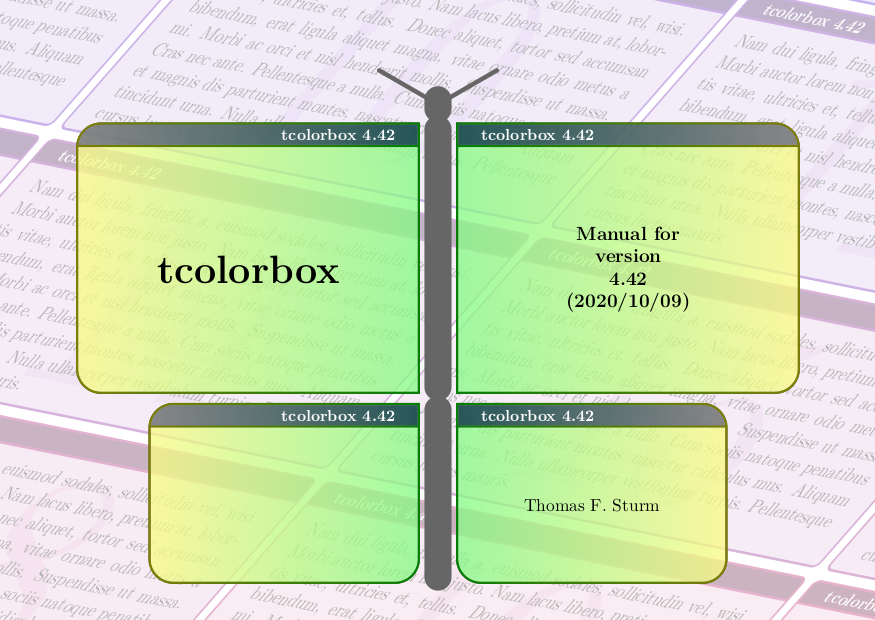
\includegraphics[width=\textwidth]{img/example-image.png}
% \end{textbox}




% \begin{textbox}{Project Gutenberg Texts}
% \begin{tabular}{r|p{0.8\textwidth}}\scriptsize
%     84 & \href{http://www.gutenberg.org/ebooks/84}{Frankenstein; Or, The Modern Prometheus by Mary Wollstonecraft Shelley} \\
%     6087 & \href{https://www.gutenberg.org/ebooks/6087}{The Vampyre; a Tale by John William Polidori} \\
%     696 & \href{https://www.gutenberg.org/ebooks/696}{The Castle of Otranto by Horace Walpole} \\
%     42 & \href{https://www.gutenberg.org/ebooks/42}{The Strange Case of Dr. Jekyll and Mr. Hyde by Robert Louis Stevenson}
% \end{tabular}

% \end{textbox}





% \begin{textbox}{Key concepts}
% \red{Bag-of-words (BOW)}


% \green{\emph{Zipf's Law}}

% \mycommand{_&§!$§/()$}{code}
% \mycommand{shutdown -h now}{to shutdown}

% \end{textbox}


% %--------------------------------------------------------------
% \section{Programming}

% \subsection{Code boxes}


% % first argument: minted programming language name, for example.. css, c, cpp, etc.
% \begin{codebox}{r}{Code box using R}
% # Install
% install.packages("tm")  # for text mining

% # Load
% library("tm")

% # text <- readLines(file.choose())
% # Read the text file from internet
% filePath <- "http://www.internet.com/text.txt"
% text <- readLines(filePath)

% \end{codebox}


% % first argument: minted programming language name, for example.. css, c, cpp, etc.
% \begin{codebox}{cpp}{Code box using C++}
% for (auto element : vector) 
% {
%     sum += element;
% }
% \end{codebox}

% \section{Graphics}
% The following is an example for a custom graphics command

% \mygraphics{img/example-image.png}



% \section{Other types of boxes}

% \begin{alerttextbox}{The Alert Block}
% \lipsum[10]
% \end{alerttextbox}

% \begin{myexampleblock}{The Example Block}
% \lipsum[22]
% \end{myexampleblock}

% \mycommand{https://github.com}{Github Link Example}

% \begin{myblock}{Branch}
% Explanation
% \end{myblock}

% \begin{myblock}{Commit}
% What's a commit?
% \end{myblock}


% \begin{myblock}{Staging}
% s. Index
% \end{myblock}


% \begin{myblock}{Lipsum}
% \lipsum[55]
% \end{myblock}

% \begin{textbox}{Yay Quotes}

% \begin{quote}
%     Yay, a quote!
% \end{quote}

% \begin{quote}
%     Yay, a longer quote! \lipsum[5]
% \end{quote}
% \end{textbox}